%
%Comparison of expected limits on cross section of BSM $\fourtops$ are shown on Figure \ref{fig:limit_BDT_vs_GNN} for two types of Asimov fits: using BDT output variable in signal regions or using GNN output variable in signal regions. The expected limits are better by ${\sim}10-20\%$ for GNN than for BDT in both compared cases (1L and 2LOS).
The expected limits on cross section of BSM $\fourtops$ using all regions (1L+2L) are shown in Figure \ref{fig:limit_all}. These are comparing to the limits obtained using only 1L regions and limits obtained using only 2L regions. \\
The previous ATLAS search for $ttH/A(\rightarrow tt)$ in the same-sign dilepton and multilepton lepton channel (SSML) shows better expected 95\% CL upper limits by a factor of two as compared to the search presented in this Note, for all assumed Higgs Boson mass in the range of [400,1000] \cite{Aad:2020klt}. The ratio of expected 95\% CL upper limits for search presented in the internal note for 1LOS to the previous search for SSML decreases from ($\approx 2.3$) for masspoint $400$ to ($\approx 1.3$) for masspoint 1000.


% No fit results with BDT possible currently (12.2.2023)
%\begin{figure}[t!]
%\centering
%\begin{subfigure}[t]{\textwidth}
%  \centering
%\begin{subfigure}[t]{0.49\textwidth}
%  \centering
%  \includegraphics[width=\textwidth]{figures/limits/GNNvsBDT_1L_withSystematics.pdf}
%  \subcaption{1L}
%  \label{fig:limit_BDT_vs_GNN_1L}
%\end{subfigure}%
%\begin{subfigure}[t]{0.49\textwidth}
%  \centering
%  \includegraphics[width=\textwidth]{figures/limits/GNNvsBDT_2L_withSystematics.pdf}
%  \subcaption{2L}
%  \label{fig:limit_BDT_vs_GNN_2L}
%\end{subfigure}
%\end{subfigure}
%\caption{Expected 95\% CL upper limits on the cross section times branching fraction to \ttbar for the production of a heavy higgs boson~\ttHA~as a function of $m_{H/A}$ for Plain Asimov fit using 1L regions (left) and 2LOS regions (right). The inner and outer bands around expected limits are the regions containing 68\% and 95\% of the distribution of limits under background-only hypothesis. Comparison is done for fits using BDT vs GNN distributions. Theoretical predictions for two values of $\tan\beta$ are shown.}
%\label{fig:limit_BDT_vs_GNN}
%\end{figure}



\begin{figure}[t!]
\centering
\begin{subfigure}[t]{0.49\textwidth}
  \centering
  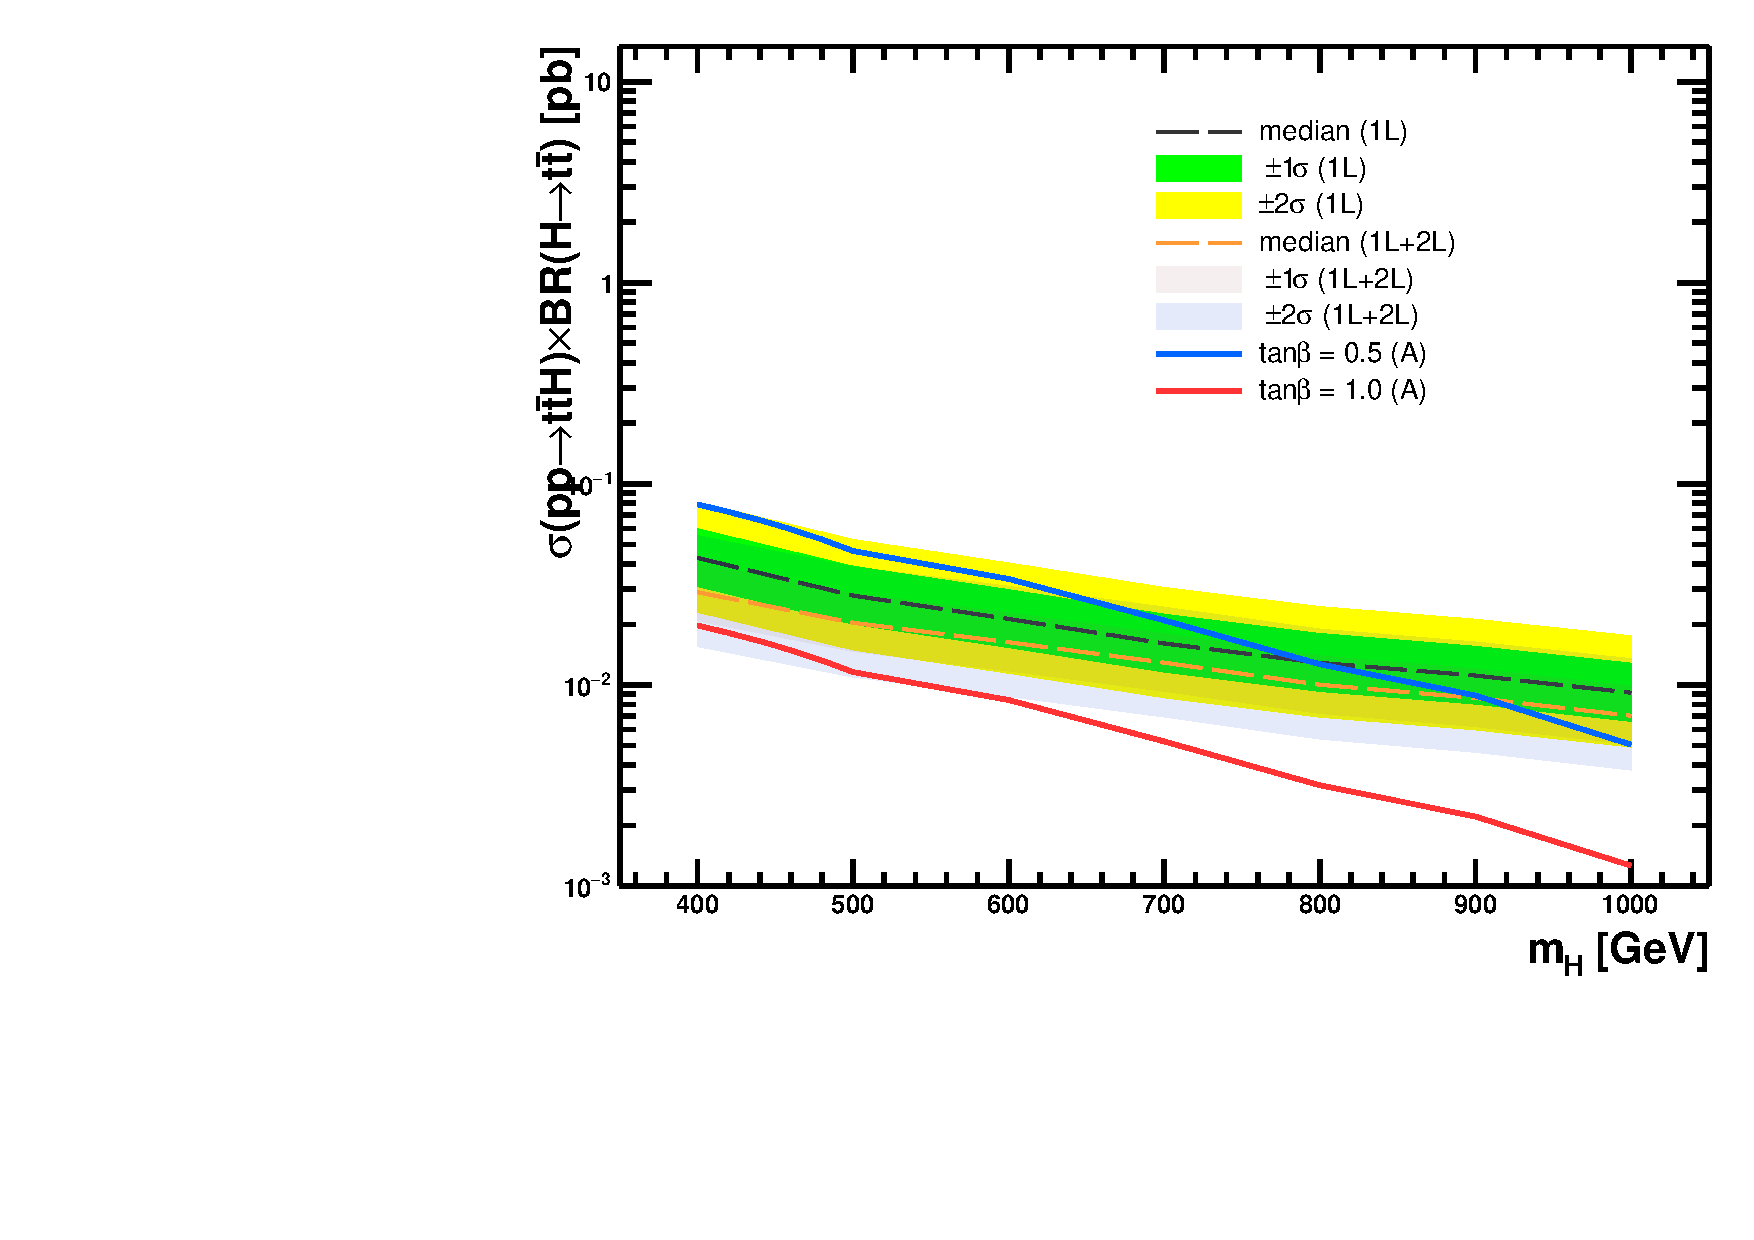
\includegraphics[width=\textwidth]{figures/limits/GNN_1LvsAll_withSystematics.pdf}
  \subcaption{1L vs combination (1L+2L)}
  \label{fig:limit_1L_vs_all}
\end{subfigure}%
\begin{subfigure}[t]{0.49\textwidth}
  \centering
  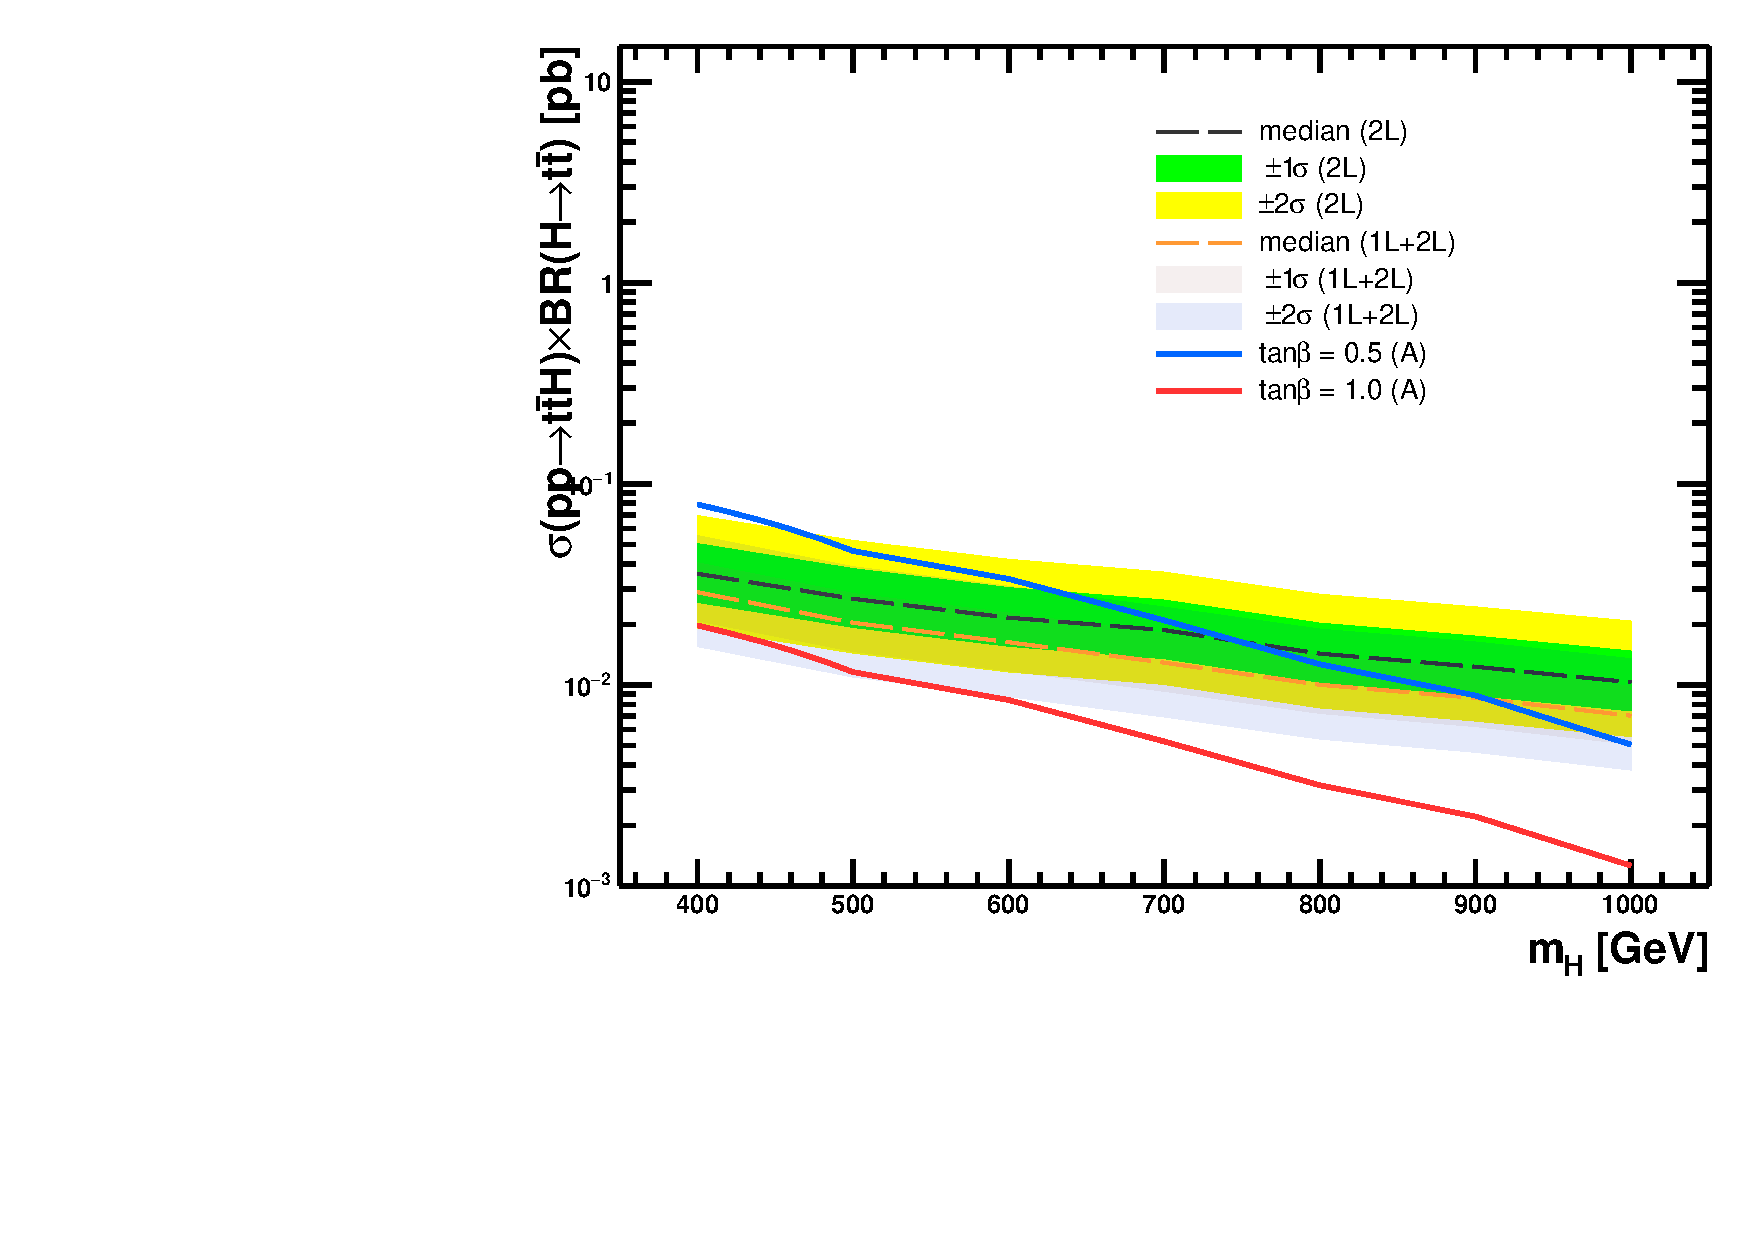
\includegraphics[width=\textwidth]{figures/limits/GNN_2LvsAll_withSystematics.pdf}
  \subcaption{2L vs combination (1L+2L)}
  \label{fig:limit_2L_vs_all}
\end{subfigure}
\caption{Comparison of the expected 95\% CL upper limits on the cross section times branching fraction to \ttbar for the production of a heavy higgs boson~\ttHA~as a function of $m_{H/A}$ for Asimov fit using all regions (1L and 2L) wrt the Asimov fit using 1L regions (left) and 2LOS regions (right). The its were done using GNNoutput distributions in the signal regions. The inner and outer bands around expected limits are the regions containing 68\% and 95\% of the distribution of limits under background-only hypothesis. Theoretical predictions for two values of $\tan\beta$ are shown.{\color{red} The current limits are wrong in these figures due to a bug for the signal normalization. The correct limits are better than the limits in these figures - it is a flat ${\sim}30\%$ effect.}}
\label{fig:limit_all}
\end{figure}
